\documentclass{article}

% if you need to pass options to natbib, use, e.g.:
     \PassOptionsToPackage{numbers, compress}{natbib}

\usepackage[preprint]{notes}

\newcommand{\ignore}[1]{}
% to avoid loading the natbib package, add option nonatbib:
\usepackage{dsfont}
\input{preamble}
\usepackage{tikz}
\usetikzlibrary{shapes.geometric, arrows}
%  \usepackage{subfigure} 
\pdfminorversion=7

%\floatname{algorithm}{Procedure}
\renewcommand{\algorithmicrequire}{\textbf{Input:}}
\renewcommand{\algorithmicensure}{\textbf{Output:}}
\newcommand{\bsl}[1]{\boldsymbol{#1}}
\newcommand{\one}[1]{\norm{#1}_{1}}
\newcommand{\bfs}[1]{\textbf{({#1}) }}
\newcommand{\typss}{\mathcal{P}_n}

\usepackage[utf8]{inputenc} % allow utf-8 input
\usepackage{microtype}      % microtypography

%\tikzstyle{input} = [rectangle, rounded corners, minimum width=1cm, minimum height=1cm,text centered, draw=black]
%\tikzstyle{process} = [rectangle, minimum width=3cm, minimum height=1cm, text centered, draw=black]
%\tikzstyle{output} = [rectangle, rounded corners, minimum width=1cm, minimum height=1cm,text centered, draw=black]
\title{Graph Theory}




\begin{document}

\maketitle

\section{Introduction and Notation}
A graph $G=(V, E)$ is specified by its \tb{vertex set}, $V$, and \tb{edge set} $E .$ In an undirected graph, the edge set is a set of unordered pairs of vertices. Unless otherwise specified, all graphs will be \tb{undirected, simple (having no loops or multiple edges) and finite.} We will sometimes assign weights to edges. These will usually be real numbers. If no weights have been specified, we view all edges as having weight $1$ . This is an arbitrary choice, and we should remember that it has an impact.

Graphs are typically used to model connections or relations between things, where "things" are vertices. However, I often prefer to think of the edges in a graph as being more important than the vertices. In this case, I may just specify an edge set $E$, and ignore the ambient vertex set.

Whenever necessary we will let $n$ denote the number of vertices. There are times that we will need to order the vertices and assign numbers to them. In this case, they will usually be $\{1, \ldots, n\}$. 

We write $\mathbb{R}^{V}$ instead of $\mathbb{R}^{n}$ to emphasize that each coordinate of the vector corresponds to a vertex of the graph.

\section{Adjacency, Diffusion and Laplacian matrix}
We can view a matrix $\boldsymbol{A}$ as providing an function that maps a vector $\boldsymbol{x}$ to the vector $\boldsymbol{A} \boldsymbol{x}$. That is, we view $\boldsymbol{A}$ as an operator. Second, I view a matrix $\boldsymbol{A}$ as providing a function that maps a vector $\boldsymbol{x}$ to a number $\boldsymbol{x}^{T} \boldsymbol{A} \boldsymbol{x} .$ That is, we also use $\boldsymbol{A}$ to define a quadratic form.
\subsection{Adjacency matrix}

\begin{defa}{\bfs{Adjacency Matrix}}
For graph $G$, its adjacency matrix is $\boldsymbol{A}_{G}$ is a \tb{symmetric} matrix, whose entries $\boldsymbol{A}_{G}(u, v)$ are given by
$$
\boldsymbol{A}_{G}(u, v)=\left\{\begin{array}{ll}
w_{u, v} = w_{v, u} & \text { if }(u, v) \in E \\
0 & \text { otherwise }
\end{array}\right.
$$
\end{defa}

\begin{rema}{\bfs{index the rows and columns using abstract $u,v$}}
We index the rows and columns of the matrix by vertices, rather than by number. The first row of a matrix has no special importance.
\end{rema}
\begin{rema}{\bfs{unweighted}}
$w_{u, v} = 1  \text { if }(u, v) \in E $
\end{rema}

\begin{rema}{\bfs{not that useful}}
While the adjacency matrix is the most natural matrix to associate with a graph, I also find it the least useful. \tb{Eigenvalues and eigenvectors are most meaningful when used to understand a natural operator or a natural quadratic form.} The adjacency matrix provides neither.
\end{rema}
\begin{rema}{\bfs{operator}}
As an operator, $\boldsymbol{A}$ acts on a vector $\boldsymbol{x} \in \mathbb{R}^{V}$ by
$$
(\boldsymbol{A x})(u)=\sum_{(u, v) \in E} w_{u, v} \boldsymbol{x}(v) .
$$
\end{rema}

\subsection{Diffusion Matrix}
\begin{defa}{\bfs{Degree of Vertex}}
We will usually write $\boldsymbol{d}(u)$ (or $d(u)$) for the degree of vertex $u$. In an \tb{unweighted} graph, the degree of a vertex is the number of edges attached to it. In the case of a weighted graph, we use the \tb{weighted} degree: the sum of the weights of the edges attached to the vertex $u$.
\end{defa}
\begin{rema}
We use $\boldsymbol{d}(u)$ because we can take it as a vector, and use $d(u)$ because we can take it as a function. We use $d(V)$ to denote the sum of the degree of the degrees of the vertices in $V$.
\end{rema}
\begin{defa}{\bfs{Diffusion Matrix}}
Let $\boldsymbol{D}_{G}$ be the diagonal matrix in which $\boldsymbol{D}_{G}(u, u)$ is the degree of vertex $u$. 
The diffusion matrix is 
$$
\boldsymbol{W}_{G}=\boldsymbol{D}_{G}^{-1} \boldsymbol{A}_{G}
$$

\end{defa}

\begin{rema}{\bfs{if $G$ is regular}}
When the graph is regular, that is when every vertex has the same degree, $\boldsymbol{W}_{G}$ is merely a rescaling of $\boldsymbol{A}_{G}$.
\end{rema}

\begin{rema}{\bfs{diffusion process}}
Imagine a process in which each vertex can contain some amount of stuff (such as a gas). At each time step, the stuff at a vertex will be uniformly distributed to its neighbors. None of the stuff that was at a vertex remains at the vertex, but stuff can enter from other vertices.
We use a vector $\bsl{p} \in \mathbb{R}^{V}$ to indicate how much stuff is at each vertex, with $\boldsymbol{p}(u)$ being the amount of stuff at vertex $u$. When describing diffusion, we will treat $\boldsymbol{p}$ as a \tb{row vector}. After one time step, the distribution of stuff at each vertex will be $\boldsymbol{p} \boldsymbol{W}_{G} .$ To see this, first consider the case when $\boldsymbol{p}$ is an elementary unit vector, $\boldsymbol{\delta}_{u}$, where I define $\boldsymbol{\delta}_{u}$ to be the vector for which $\boldsymbol{\delta}_{u}(u)=1$ and for every other vertex $v, \boldsymbol{\delta}_{u}(v)=0 .$ The vector $\boldsymbol{\delta}_{u} \boldsymbol{D}_{G}^{-1}$ has the value $1 / \boldsymbol{d}(u)$ at vertex $u$, and is zero everywhere else. So, the vector $\boldsymbol{\delta}_{u} \boldsymbol{D}_{G}^{-1} A_{G}$ has value $1 / \boldsymbol{d}(u)$ at every vertex $v$ that is a neighbor of $u$, and is zero everywhere else.
\end{rema}
\begin{rema}
The spectral theory provides a good understanding of what happens when one \tb{repeatedly} applies a linear operator like $\boldsymbol{W}_{G}$.
\end{rema}
\subsection{Laplacian Matrix}
\begin{defa}{\bfs{Laplacian Matrix}}\label{matrix:lp}
$$
\boldsymbol{L}_{G}\coloneqq \boldsymbol{D}_{G}-\boldsymbol{A}_{G}
$$
\end{defa}

\begin{rema}{\bfs{most natural quadratic form}}
The most natural quadratic form associated with a graph is defined in terms of its Laplacian matrix.
Given any \tb{function} on the vertices, $\boldsymbol{x} \in \mathbb{R}^{V}$, the Laplacian quadratic form is
\begin{align}
\boldsymbol{x}^{T} \boldsymbol{L}_{G} \boldsymbol{x}=\sum_{(u, v) \in E} w_{u, v}(\boldsymbol{x}(u)-\boldsymbol{x}(v))^{2} \label{matrix:lpeq1}
\end{align}
This form measures the \tb{smoothness} of the function $\boldsymbol{x} .$ It will be small if the function $\boldsymbol{x}$ does not jump too much over any edge. Note here function means instead of taking $\bsl{x}$ as a vector,  we takes $\bsl{x}(\cdot)$ as a function with the vertex $V$ as the domain. In other words, $\bsl{x}: V \rightarrow \mathbb{R}$.
\end{rema}

\begin{rema}{\bfs{positive semidefinite}}\label{matrix:lpremapos}
%Even if $w_{u, v}\ne w_{v, u}$ in \cref{matrix:lpeq1}, we may view it as a symmetric matrix in the quadratic form since \cref{matrix:lpeq1} is equivalent to $\sum_{(u, v) \in E} \frac{w_{u, v}+w_{u, v}}{2}(\boldsymbol{x}(u)-\boldsymbol{x}(v))^{2}$. 
Note here it does not contain  $w_{u, v}$ and $w_{v, u}$ twice. 
From \cref{matrix:lpeq1}, we know it is positive semidefinite with nonnegative eigenvalues since $w_{u, v}\ge 0$. Therefore the smallest eigenvalue $\lambda_1\ge 0$ and by setting $\bsl{x}=\indicatore{}$, we have the conclusion that the smallest eigenvalue $\lambda_1 = 0$.
\end{rema}

\tb{Decomposition of Laplacian Matrix (alternative definition of Laplacian matrix):}

We can take the quadratic form 
\begin{align}
    \sum_{(u, v) \in E} w_{u, v}(\boldsymbol{x}(u)-\boldsymbol{x}(v))^{2} \label{matrix:2lpeq}
\end{align} for $\bsl{x}$ as an alternative definition for Laplacian matrix, where we view it as a mapping that takes vector $\bsl{x}$ to $\Real{+}$. The mapping \cref{matrix:2lpeq} is equivalent to setting $\boldsymbol{x}^{T} \boldsymbol{L}_{G} \boldsymbol{x}$ with $\boldsymbol{L}_{G} = \boldsymbol{D}_{G}-\boldsymbol{A}_{G}$

We next show the equivalence. 

\tb{1.) graph $G_{1,2}$ with only two nodes:}

Consider a graph with just two vertices and one edge. Let's call it $G_{1,2}$. Consider the vector $\boldsymbol{\delta}_{1}-\boldsymbol{\delta}_{2}$, we have
$$
\boldsymbol{x}(1)-\boldsymbol{x}(2)=\boldsymbol{\delta}_{1}^{T} \boldsymbol{x}-\boldsymbol{\delta}_{2}^{T} \boldsymbol{x}=\left(\boldsymbol{\delta}_{1}-\boldsymbol{\delta}_{2}\right)^{T} \boldsymbol{x}
$$
so
$$
(\boldsymbol{x}(1)-\boldsymbol{x}(2))^{2}=\left(\left(\boldsymbol{\delta}_{1}-\boldsymbol{\delta}_{2}\right)^{T} \boldsymbol{x}\right)^{2}=\boldsymbol{x}^{T}\left(\boldsymbol{\delta}_{1}-\boldsymbol{\delta}_{2}\right)\left(\boldsymbol{\delta}_{1}-\boldsymbol{\delta}_{2}\right)^{T} \boldsymbol{x}=\boldsymbol{x}^{T}\left[\begin{array}{rr}
1 & -1 \\
-1 & 1
\end{array}\right] \boldsymbol{x}
$$
So, we have get the \tb{existence} that we have
$$
\boldsymbol{x}^{T} \boldsymbol{L}_{G_{1,2}} \boldsymbol{x}=(\boldsymbol{x}(1)-\boldsymbol{x}(2))^{2}
$$ with 
$$
\boldsymbol{L}_{G_{1,2}}=\left[\begin{array}{rr}
1 & -1 \\
-1 & 1
\end{array}\right]
$$
The uniqueness comes from the choosing $\bsl{x}$ as $\boldsymbol{\delta}_{1}$, $\boldsymbol{\delta}_{2}$ and $\boldsymbol{\delta}_{1}-\boldsymbol{\delta}_{2}$.

\tb{1.) general graph:}

Now, let $G_{u, v}$ be the graph with just one edge between $u$ and $v .$ It can have as many other vertices as you like. The Laplacian of $G_{u, v}$ can be written in the same way: $\boldsymbol{L}_{G_{u, v}}=\left(\boldsymbol{\delta}_{u}-\boldsymbol{\delta}_{v}\right)\left(\boldsymbol{\delta}_{u}-\boldsymbol{\delta}_{v}\right)^{T}$.
This is the matrix that is zero except at the intersection of rows and columns indexed by $u$ and $v$, where it looks looks like
$$
\left[\begin{array}{rr}
1 & -1 \\
-1 & 1
\end{array}\right]
$$
From the linearity, we have that \cref{matrix:2lpeq} equals
$$\bsl{x}^T\sum_{(u, v) \in E} w_{u, v}\left(\boldsymbol{\delta}_{u}-\boldsymbol{\delta}_{v}\right)\left(\boldsymbol{\delta}_{u}-\boldsymbol{\delta}_{v}\right)^{T}\bsl{x}=\bsl{x}^T\sum_{(u, v) \in E} w_{u, v} \boldsymbol{L}_{G_{u, v}}\bsl{x}.
$$
We can therefore let
$$
\boldsymbol{L}_{G}=\sum_{(u, v) \in E} w_{u, v} \boldsymbol{L}_{G_{u, v}}.
$$
which agrees with the definition of the Laplacian from \cref{matrix:lp}:
$$
\boldsymbol{L}_{G}=\boldsymbol{D}_{G}-\boldsymbol{A}_{G}
$$
where
$$
\boldsymbol{D}_{G}(u, u)=\sum_{v} w_{u, v}
$$
The The uniqueness comes from the if $\exists \boldsymbol{L}'_{G}\ne \boldsymbol{L}_{G}$, we need $\bsl{x}^T(\boldsymbol{L}'_{G}- \boldsymbol{L}_{G})\bsl{x} \equiv 0$, which is not possible if $\boldsymbol{L}'_{G}\ne \boldsymbol{L}_{G}$.

\begin{rema}{\bfs{$\boldsymbol{L}_{G}$ as operator}}\label{matrix:lgop}
The formula  in \cref{matrix:2lpeq} turns out to be useful when we view the Laplacian as an \tb{operator}. For every vector $\boldsymbol{x}$ we have
$$
\left(\boldsymbol{L}_{G} \boldsymbol{x}\right)(u)=\bsl{d(u)} \boldsymbol{x}(u)-\sum_{(u, v) \in E} w_{u, v} \boldsymbol{x}(v)=\sum_{(u, v) \in E} w_{u, v}(\boldsymbol{x}(u)-\boldsymbol{x}(v))
$$
\end{rema}


\section{Special Graph}
We list some examples of graphs which may be studied in this notes:
\begin{enumerate}
    \item The \tb{path} $P_n$ on $n$ vertices. The vertices are $\{1, \ldots n\}$. The edges are $(i, i+1)$ for $1 \leq i<n$.
    \item The \tb{ring} on $n$ vertices. The vertices are $\{1, \ldots n\}$. The edges are all those in the path, plus the edge $(1, n)$.
    \item The \tb{hypercube} $H_k$ on $2^{k}$ vertices. The vertices are elements of $\{0,1\}^{k}$. Edges exist between vertices that differ in only one coordinate.
    \item The \tb{complete graph} $K_{n}$ on $n$ vertices, which has edge set $\{(u, v): u \neq v\}$.
    \item  The \tb{star graph} $S_{n}$ on $n$ vertices, which has edge set $\{(1, u): 2 \leq u \leq n\}$.
    \item The \tb{regular graph}, where every vertex has the same degree,
\end{enumerate}


\section{Eigenvalues and Eigenvectors of the Laplacian}

We order the $n$ eigenvalue of the Laplacian $\bsl{L}_G$ as $\lambda_1\le \lambda_2\le\ldots \le \lambda_n$ with corresponding eigenvectors $\boldsymbol{\psi}_1,\boldsymbol{\psi}_2,\ldots,\boldsymbol{\psi}_n$.  The different order of vertex, and corresponding different representation of  $\bsl{L}_G$  does not affect the eigenvalues since $\bP^T\bsl{L}_G\bP$ with permutation matrix $\bP$ is a special similarity and does not affect the eigenvalues. We have mentioned in \cref{matrix:lpremapos}, $\lambda_1=0$ with the eigenvector of $\lambda_1$ as $\indicatore{}$.


\begin{rema}{\bfs{$\lambda_n$: the highest vibration frequency}}
The $n$-th eigenvalue $\lambda_n$ is the largest eigenvalue the Laplacian, corresponds to the highest vibration frequency  in a graph. Its corresponding eigenvector $\boldsymbol{\psi}_n$ tries to assign as different as possible values to neighboring vertices. Please understand this using $\bsl{L}_G=\lambda_1\boldsymbol{\psi}_1\boldsymbol{\psi}_2^T+\lambda_2 \boldsymbol{\psi}_2\boldsymbol{\psi}_2^T+\ldots+\lambda_n\boldsymbol{\psi}_n\boldsymbol{\psi}_n^T$ or use the Rayleigh quotient.
\end{rema}

\subsection{Examples}

\begin{lema}{\bfs{Complete Graph $K_n$}}
The Laplacian of $K_{n}$ has eigenvalue 0 with multiplicity 1 and $n$ with multiplicity $n-1$
\end{lema}
\begin{proof}
To compute the non-zero eigenvalues, let $\bsl{\psi}$ be any non-zero vector orthogonal to the all-$1$s vector $\indicatore{}$, so
$$
\sum_{u} \bsl{\psi}(u)=0
$$
We now compute the first coordinate of $\boldsymbol{L}_{K_{n}} \boldsymbol{\psi} .$ Using \cref{matrix:lgop}, we find
$$
\left(\boldsymbol{L}_{K_{n}} \boldsymbol{\psi}\right)(1)=\sum_{v \geq 2}(\boldsymbol{\psi}(1)-\boldsymbol{\psi}(v))=(n-1) \boldsymbol{\psi}(1)-\sum_{v=2}^{n} \boldsymbol{\psi}(v)=n \boldsymbol{\psi}(1), \quad \text { by }(2.6)
$$
As the choice of coordinate was arbitrary, we have $\boldsymbol{L} \boldsymbol{\psi}=n \boldsymbol{\psi}$. So, every vector orthogonal to the all-1s vector is an eigenvector of eigenvalue $n$.
\end{proof}
\begin{rema}{\bfs{Alternative approach}}
Observe that $\boldsymbol{L}_{K_{n}}=n \boldsymbol{I}-\mathbf{1 1}^{T}$. Use Brauer’s theorem in \cite[Page51]{horn2012matrix}
\end{rema}

To determine the eigenvalues of $S_{n}$, we first observe that each vertex $i \geq 2$ has degree 1 , and that each of these degree-one vertices has the same neighbor. Whenever two degree-one vertices share the same neighbor, they provide an eigenvector of eigenvalue $1 .$
\begin{lema}\label{eilp:lem2}
Let $G=(V, E)$ be a graph, and let $v$ and $w$ be vertices of degree one that are both connected to another vertex $z .$ Then, vector $\boldsymbol{\psi}=\boldsymbol{\delta}_{v}-\boldsymbol{\delta}_{w}$ is an eigenvector of $\boldsymbol{L}_{G}$ of eigenvalue 1 .
\end{lema}

\begin{proof}
Just multiply $\boldsymbol{L}_{G}$ by $\boldsymbol{\psi}$, and check vertex-by-vertex that it equals $\boldsymbol{\psi} .$
\end{proof}

\begin{lema}{\bfs{Star Graph $S_n$}}
The graph $S_{n}$ has eigenvalue $0$ with multiplicity $1$ (from connectivity), eigenvalue 1 with multiplicity $n-2$ (from \cref{eilp:lem2}), and eigenvalue $n$ with multiplicity $1 .$
\end{lema} 

\begin{proof}
Applying \cref{eilp:lem2} to vertices $i$ and $i+1$ for $2 \leq i<n$, we find $n-2$ linearly independent eigenvectors of the form $\boldsymbol{\delta}_{i}-\boldsymbol{\delta}_{i+1}$, all with eigenvalue $1 .$ As 0 is also an eigenvalue, only one eigenvalue remains to be determined. We could then use trace to get it is $n$. Eigenvector is also easy since we know the final eigenvector of eigenvalue $n$ must have the same value for vertex $2$ to $n$ (from orthogonal to $\boldsymbol{\delta}_{v}-\boldsymbol{\delta}_{w}$) and to determine the first element, we use that it is orthogonal to $\indicatore{}$.
\end{proof} 
\begin{lema}{\bfs{Hypercube $H_d$}}
 $H_{d}$ has eigenvalues $2 i$ for $i \in\{0,1, \ldots, d\}$, and that the eigenvalue $2 i$ has multiplicity $\left(\begin{array}{l}d \\ i\end{array}\right) .$  $H_{d}$ has a basis of eigenvectors of the form $\bsl{\psi}_{a}(b)=(-1)^{a^{T} b}$,
where $a,b \in\{0,1\}^{d}$. The eigenvalue of which $\boldsymbol{\psi}_{a}$ is an eigenvector is the number of ones in $\boldsymbol{\psi}_{a}$.
\end{lema}
\begin{proof}
Directly from \cref{gp:thm1} using the fact that the non-zero eigenvector of $\boldsymbol{L}_{G}$ is $(1,-1)$, where $G$ be the graph with vertex set $\{0,1\}$ and one edge between those vertices, with eigenvalue $2$.
\end{proof}

\subsection{Graph Product}

\begin{defa}{\bfs{Graph Product}}
Let $G=(V, E)$ and $H=(W, F)$ be graphs. Then $G \times H$ is the graph with vertex set $V \times W$ and edge set
$$
\begin{array}{l}
((v, w),(\hat{v}, w)) \text { where }(v, \hat{v}) \in E \text { and } \\
((v, w),(v, \hat{w})) \text { where }(w, \hat{w}) \in F
\end{array}
$$
\end{defa} 
\begin{rema}{\bfs{hypercube graph}}
Let $G$ be the graph with vertex set $\{0,1\}$ and one edge between those vertices. It's Laplacian matrix has eigenvalues 0 and $2 .$ You should check that $H_{1}=G$ and that $H_{d}=H_{d-1} \times G$.
\end{rema}


\begin{thma}{\bfs{Eigenvalues and Eigenvetors of Producted Graph }}\label{gp:thm1}
Let $G=(V, E)$ and $H=(W, F)$ be graphs with Laplacian eigenvalues $\lambda_{1}, \ldots, \lambda_{n}$ and $\mu_{1}, \ldots, \mu_{m}$, and eigenvectors $\boldsymbol{\alpha}_{1}, \ldots, \boldsymbol{\alpha}_{n}$ and $\boldsymbol{\beta}_{1}, \ldots, \boldsymbol{\beta}_{m}$, respectively. Then, for
each $1 \leq i \leq n$ and $1 \leq j \leq m,$ the Laplacian of $G \times H$, $\bsl{L}_{G \times H}$, has an eigenvector $\bsl{\gamma}_{i, j}$ of eigenvalue $\lambda_{i}+\mu_{j}$ such that
$$
\boldsymbol{\gamma}_{i, j}(v, w)=\boldsymbol{\alpha}_{i}(v) \boldsymbol{\beta}_{j}(w)
$$
\end{thma}
\begin{proof}
 Let $\boldsymbol{\alpha}$ be an eigenvector of $\bsl{L} _{G}$ of eigenvalue $\lambda$, let $\boldsymbol{\beta}$ be an eigenvector of $\bsl{L} _{H}$ of eigenvalue
$\mu$, and let $\bsl{\gamma}$ be defined as above.
To see that $\bsl{\gamma}$ is an eigenvector of eigenvalue $\lambda+\mu$, we compute
$$
\begin{aligned}
(\bsl{L} \bsl{\gamma})(u, v) &=\sum_{(\hat{u}, v):(u, \hat{u}) \in E}(\bsl{\gamma}(u, v)-\bsl{\gamma}(\hat{u}, v))+\sum_{(u, \hat{v}):(v, \hat{v}) \in F}(\bsl{\gamma}(u, v)-\bsl{\gamma}(u, \hat{v})) \\
&=\sum_{(\hat{u}, v):(u, \hat{u}) \in E}(\boldsymbol{\alpha}(u) \boldsymbol{\beta}(v)-\boldsymbol{\alpha}(\hat{u}) \boldsymbol{\beta}(v))+\sum_{(u, \hat{v}):(v, \hat{v}) \in F}(\boldsymbol{\alpha}(u) \boldsymbol{\beta}(v)-\boldsymbol{\alpha}(u) \boldsymbol{\beta}(\hat{v})) \\
&=\sum_{(\hat{u}, v):(u, \hat{u}) \in E} \boldsymbol{\beta}(v)(\boldsymbol{\alpha}(u)-\boldsymbol{\alpha}(\hat{u}))+\sum_{(u, \hat{v}):(v, \hat{v}) \in F} \boldsymbol{\alpha}(u)(\boldsymbol{\beta}(v)-\boldsymbol{\beta}(\hat{v})) \\
&=\boldsymbol{\beta}(v) \lambda \boldsymbol{\alpha}(u)+\boldsymbol{\alpha}(u) \mu \boldsymbol{\beta}(v) \\
&=(\lambda+\mu)(\boldsymbol{\alpha}(u) \boldsymbol{\beta}(v)) .
\end{aligned}
$$
\end{proof}



\subsection{Isoperimetry and $\lambda_{2}$}
\tb{keywords:} cutting, partitioning, and clustering graphs.

One can also show that \tb{$\lambda_{2}>0$ if and only if the graph is connected.} If the graph is disconnected, one can construct at least two orthogonal vectors with eigenvalue zero: consider vectors that are constant on one component of the graph and zero everywhere else. On the other hand, if the graph is connected then we can show that $\lambda_{2}>0$ : Let $\boldsymbol{x}$ be any vector orthogonal to the constant vectors. So, there must be two vertices $u$ and $v$ for which $\boldsymbol{x}(u) \neq \boldsymbol{x}(v) .$ As there is a path between these vertices, there must be some edge across which $\boldsymbol{x}$ changes value. So, the quadratic form will be positive on $\boldsymbol{x}$.

We will show $\lambda_{2}$ intimately related to the problem of dividing a graph into two pieces without cutting too many edges.

\begin{defa}{\bfs{Boundary}}
Let $S$ be a subset of the vertices of a graph. One way of measuring how well $S$ can be separated from the graph is to count the number of edges connecting $S$ to the rest of the graph. These edges are called the boundary $\partial(S)$ of $S$:
$$
\partial(S) \stackrel{\text { def }}{=}\{(u, v) \in E: u \in S, v \notin S\}
$$
\end{defa}
\begin{defa}{\bfs{Isoperimetric Ratio}} The ratio of the total number of edges on the boundary to the size of $S$ is called isoperimetric ratio $\theta(S)$:
$$
\theta(S)\coloneqq \frac{|\partial(S)|}{|S|}
$$
\end{defa}
\begin{defa}{\bfs{Isoperimetric Number }}
The isoperimetric number $\theta_{G}$ of a graph is the minimum isoperimetric ratio over all sets of at most half the vertices:
$$
\theta_{G} \coloneqq \min _{|S| \leq n / 2} \theta(S) .
$$
\end{defa}

We will now derive a lower bound on $\theta_{G}$ in terms of $\lambda_{2}$. We will present an upper bound, known as Cheeger's Inequality later.
\begin{thma}{\bfs{Lower Bound on $\theta_{G}$ w.r.t. $\lambda_{2}$}}\label{lp:thmlower}
For every $S \subset V$
$$
\theta(S) \geq \lambda_{2}(1-s)
$$
where $s=|S| /|V| .$ In particular,
$$
\theta_{G} \geq \lambda_{2} / 2
$$
\end{thma} 
\begin{rema}{\bfs{Upper Bound on $\theta_{G}$ }}\label{lp:thmlower}
See Cheeger’s Inequality in \cref{sec:cnc}.
\end{rema}
\begin{proof}
$$
\lambda_{2}=\min _{\boldsymbol{x}: \boldsymbol{x}^{T} \mathbf{1}=0} \frac{\boldsymbol{x}^{T} \boldsymbol{L}_{G} \boldsymbol{x}}{\boldsymbol{x}^{T} \boldsymbol{x}}
$$
for every non-zero $\boldsymbol{x}$ orthogonal to $\mathbf{1}$ we know that
$$
\boldsymbol{x}^{T} \boldsymbol{L}_{G} \boldsymbol{x} \geq \lambda_{2} \boldsymbol{x}^{T} \boldsymbol{x}
$$

To exploit this inequality, we need a vector related to the set $S .$ A natural choice is $\chi_{S}$, the characteristic vector of $S$,
$$
\chi_{S}(u)=\left\{\begin{array}{ll}
1 & \text { if } u \in S \\
0 & \text { otherwise }
\end{array}\right.
$$
We find
$$
\boldsymbol{\chi}_{S}^{T} \boldsymbol{L}_{G} \boldsymbol{\chi}_{S}=\sum_{(u, v) \in E}\left(\boldsymbol{\chi}_{S}(u)-\boldsymbol{\chi}_{S}(v)\right)^{2}=|\partial(S)|
$$
However, $\chi_{S}$ is not orthogonal to 1 . To fix this, use
$$
\boldsymbol{x}=\boldsymbol{\chi}_{S}-s \mathbf{1}
$$
SO
$$
\boldsymbol{x}(u)=\left\{\begin{array}{ll}
1-s & \text { for } u \in S, \text { and } \\
-s & \text { otherwise }
\end{array}\right.
$$
We have $\boldsymbol{x}^{T} \mathbf{1}=0$, and
$$
\boldsymbol{x}^{T} \boldsymbol{L}_{G} \boldsymbol{x}=\sum_{(u, v) \in E}\left(\left(\boldsymbol{\chi}_{S}(u)-s\right)-\left(\boldsymbol{\chi}_{S}(v)-s\right)\right)^{2}=|\partial(S)|
$$
To finish the proof, we compute
$$
\boldsymbol{x}^{T} \boldsymbol{x}=|S|(1-s)^{2}+(|V|-|S|) s^{2}=|S|\left(1-2 s+s^{2}\right)+|S| s-|S| s^{2}=|S|(1-s) .
$$
\end{proof}

\begin{rema}
If $\lambda_{2}$ is big, then $G$ is very well connected: the boundary of every small set of vertices is at least $\lambda_{2}$ times $(1-\frac{|S|}{|V|})|S|$ which slightly smaller than the number of vertices $|S|$.
\end{rema}
We will use the computation in the last line of that proof often, so we will make it a claim.
\begin{cora}
Let $S \subseteq V$ have size $s|V| .$ Then
$$
\left\|\boldsymbol{\chi}_{S}-s \mathbf{1}\right\|^{2}=s(1-s)|V|
$$
\end{cora} 

\begin{cora}
For hypercube $H_d$, $\theta_{H_{d}} \geq 1$.
In particular, for every set of at most half the vertices of the hypercube, the number of edges on the boundary of that set is at least the number of vertices in that set.
\end{cora}
\begin{proof}
It follows directly from $\lambda_2(H_d) =2$.
\end{proof}


\section{Eigenvalues and Eigenvectors of the Adjacency}
We order the $n$ eigenvalue of the adjacency $\bsl{A}_G$ as $\mu_1\ge \mu_2\ge\ldots \ge \mu_n$. 
\begin{rema}
The reason for this convention is so that $\mu_{i}$ corresponds to the $i$-th Laplacian eigenvalue $\lambda_{i} .$ If $G$ is a $d$-regular graph, then $\boldsymbol{D}=\boldsymbol{I} d$, and
$$
\boldsymbol{L}=\boldsymbol{I} d-\boldsymbol{A}
$$
and so
$$
\lambda_{i}=d-\mu_{i}
$$
So, we see that the largest adjacency eigenvalue of a $d$ -regular graph is $d$, and its corresponding eigenvector is the constant vector. Note the translate as in \cite[Page57]{horn2012matrix} 
\end{rema}

\subsection{The Largest Eigenvalue, $\mu_{1}$}
We now examine $\mu_{1}$ for graphs which are \tb{not necessarily regular}. Let $G$ be a graph, let $d_{\max }$ be the maximum degree of a vertex in $G$, and let $d_{\text {ave }}$ be the average degree of a vertex in $G$. If the graph is weighted, then these are the weighted degrees. In the following, we let $d(u)$ denote the (weighted) degree of vertex $u$.
\begin{lema}{\bfs{Upper and Lower Bounds for $\mu_1$}}
 $$
d_{\text {ave }} \leq \mu_{1} \leq d_{\text {max }}
$$
\end{lema}

\begin{proof}
While this theorem holds in the weighted case, we just prove it in the unweighted case for simplicity.
The lower bound follows by considering the Rayleigh quotient with the all-1s vector:
$$
\mu_{1}=\max _{x} \frac{\boldsymbol{x}^{T} \boldsymbol{A} \boldsymbol{x}}{\boldsymbol{x}^{T} \boldsymbol{x}} \geq \frac{\mathbf{1}^{T} \boldsymbol{A} \mathbf{1}}{\mathbf{1}^{T} \mathbf{1}}=\frac{\sum_{(u, v) \in E} \boldsymbol{A}(u, v)}{n}=\frac{\sum_{u} \boldsymbol{d}(u)}{n} .
$$
To prove the upper bound, Let $\boldsymbol{\phi}_{1}$ be an eigenvector of eigenvalue $\mu_{1}$. Let $v$ be the vertex on which it takes its maximum value, so $\boldsymbol{\phi}_{1}(v) \geq \boldsymbol{\phi}_{1}(u)$ for all $u$, and assume without loss of generality that $\boldsymbol{\phi}_{1}(v) \neq 0 .$ We have
\begin{align}
   \mu_{1}=\frac{\left(A \boldsymbol{\phi}_{1}\right)(v)}{\boldsymbol{\phi}_{1}(v)}=\frac{\sum_{u:(u, v) \in E} \boldsymbol{\phi}_{1}(u)}{\boldsymbol{\phi}_{1}(v)}=\sum_{u:(u, v) \in E} \frac{\boldsymbol{\phi}_{1}(u)}{\boldsymbol{\phi}_{1}(v)} \le \sum_{u:(u, v) \in E} 1 = d(v) = d_{\max } \label{aj:eq1}
\end{align}

\end{proof}
We can strengthen the lower bound by proving that $\mu_{1}$ is at least the averge degree of every subgraph of $G$

\begin{lema}{\bfs{Improved Lower Bounds}}\label{aj:lema2}
  For every $S \subseteq V$, let $d_{\text {ave }}(S)$ be the average degree of vertices in the subgraph induced on the vertices in $S$ (that is, having only edges between vertices of $S) .$ Then,
$$
d_{a v e}(S) \leq \mu_{1}
$$
\end{lema} 


\begin{lema}
  Let $\boldsymbol{A}$ be a symmetric matrix and let $S$ be a subset of its row and column indices. Let $\boldsymbol{A}(S)$ denote the sub-matrix of $\boldsymbol{A}$ with rows and columns indexed by $S$. Then
$$
\lambda_{\max }(\boldsymbol{A}) \geq \lambda_{\max }(\boldsymbol{A}(S)) \geq \lambda_{\min }(\boldsymbol{A}(S)) \geq \lambda_{\min }(\boldsymbol{A})
$$
\end{lema}
\begin{proof}
It suffices to the lemma in the case that $S=\{1, \ldots, n-1\} .$ So, let $S=\{1, \ldots, n-1\}$ and let $\boldsymbol{B}=\boldsymbol{A}(S)$
For any vector $\boldsymbol{y} \in \mathbb{R}^{n-1}$, we have
$$
\boldsymbol{y}^{T} \boldsymbol{B} \boldsymbol{y}=\left(\begin{array}{l}
\boldsymbol{y} \\
0
\end{array}\right)^{T} \boldsymbol{A}\left(\begin{array}{l}
\boldsymbol{y} \\
0
\end{array}\right)
$$
So, for $\boldsymbol{y}$ an eigenvector of $\boldsymbol{B}$ of eigenvalue $\lambda_{\max }(\boldsymbol{B})$,
$$
\lambda_{\max }(\boldsymbol{B})=\frac{\boldsymbol{y}^{T} \boldsymbol{B} \boldsymbol{y}}{\boldsymbol{y}^{T} \boldsymbol{y}}=\frac{\left(\begin{array}{l}
\boldsymbol{y} \\
0
\end{array}\right)^{T} \boldsymbol{A}\left(\begin{array}{l}
\boldsymbol{y} \\
0
\end{array}\right)}{\left(\begin{array}{l}
\boldsymbol{y} \\
0
\end{array}\right)^{T}\left(\begin{array}{l}
\boldsymbol{y} \\
0
\end{array}\right)} \leq \max _{\boldsymbol{x} \in \mathbb{R}^{n}} \frac{\boldsymbol{x}^{T} \boldsymbol{A} \boldsymbol{x}}{\boldsymbol{x}^{T} \boldsymbol{x}}=\lambda_{\max }(\boldsymbol{A})
$$
The same argument works for the smallest eigenvalues.
\end{proof}
\begin{proof} (of \cref{aj:lema2})
Let $S \subseteq V$, and let $G(S)$ denote the subgraph induced on the vertices in $S$. If $\boldsymbol{A}$ is the adjacency matrix of $G$, then $\boldsymbol{A}(S)$ is the adjacency matrix of $G(S) .$ Lemma $3.3 .1$ says that $d_{\text {ave }}(S)$ is at most the largest eigenvalue of the adjacency matrix of $G(S)$, and Lemma 3.3.3 says that this is at most $\mu_{1}$.
\end{proof}  
\begin{lema}
  If $G$ is connected and $\mu_{1}=d_{\text {max }}$, then $G$ is $d_{\text {max }}$-regular.
\end{lema} 
\begin{proof}
If we have equality in \cref{aj:eq1}, then it must be the case that $\bsl{d}(v)=d_{\max }$ and $\boldsymbol{\phi}_{1}(u)=\bsl{\phi}_{1}(v)$ for all $(u, v) \in E .$ Thus, we may apply the same argument to every neighbor of $v .$ As the graph is connected, we may keep applying this argument to neighbors of vertices to which it has already been applied to show that $\bsl{\phi}_{1}(z)=\bsl{\phi}_{1}(v)$ and $\bsl{d}(z)=d_{\max }$ for all $z \in V$.
\end{proof}  
\begin{rema}{\bfs{spreading property}}
Same proof technique of the spreading property in as in \cite[Page397]{horn2012matrix} 
\end{rema}
\subsection{More Property of Eigenvalues and Eigenvectors}
Since I'm familiar of the theorems and lemmas, I just list them here without any proof. A connected weighted graph $G$ has a irreducible nonnegative adjacency matrix.

\begin{lema}{\bfs{Perron-Frobenius, Symmetric Case}}
  Let $G$ be a connected weighted graph, let $\boldsymbol{A}$ be its adjacency matrix, and let $\mu_{1} \geq \mu_{2} \geq \cdots \geq \mu_{n}$ be its eigenvalues. Then
  \begin{enumerate}
      \item $\mu_{1} \geq-\mu_{n}$
      \item $\mu_{1}>\mu_{2}$
      \item The eigenvalue $\mu_{1}$ has a strictly positive eigenvector.
  \end{enumerate}
\end{lema} 
\begin{rema}
$\mu_{1}>\mu_{2}$ comes from that $\rho(A)>0$ and is algebraically simple eigenvalue of $A$. For non-symmetric $A$ we do not have uniqueness, however since here $A$ is  symmetric and only have real eigenvalue, we then have the uniqueness. See also \cite[534]{horn2012matrix}
\end{rema}

\begin{lema}
  Let $G$ be a connected weighted graph (with non-negative edge weights), let $\boldsymbol{A}$ be its adjacency matrix, and assume that some non-negative vector $\bsl{\phi}$ is an eigenvector of $\boldsymbol{A} .$ Then, $\boldsymbol{\phi}$ is strictly positive.
\end{lema} 

\begin{lema}
  If $G$ is a unweighted connected graph, then $\mu_{n}=-\mu_{1}$ if and only if $G$ is bipartite.
\end{lema}
\begin{proof}
First, assume that $G$ is bipartite. That is, we have a decomposition of $V$ into sets $U$ and $W$ such that all edges go between $U$ and $W .$ Let $\bsl{\phi}_{1}$ be the eigenvector of $\mu_{1}$. Define
$$
\boldsymbol{x}(u)=\left\{\begin{array}{ll}
\boldsymbol{\phi}_{1}(u) & \text { if } u \in U, \text { and } \\
-\boldsymbol{\phi}_{1}(u) & \text { if } u \in W
\end{array}\right.
$$
For $u \in U$, we have
$$
\\
(\boldsymbol{A} \boldsymbol{x})(u)=\sum_{(u, v) \in E} \boldsymbol{x}(v)=-\sum_{(u, v) \in E} \boldsymbol{\phi}(v) \stackrel{\stackrel{\mathbf{A} \bsl{\phi}_{1}=\mu_{1} \bsl{\phi}_{1}}{\downarrow}}{=}-\mu_{1} \boldsymbol{\phi}(u)=-\mu_{1} \boldsymbol{x}(u) .
$$
Using a similar argument for $u \notin U$, we can show that $\bsl{x}$ is an eigenvector of eigenvalue $-\mu_{1}$.
To go the other direction, assume that $\mu_{n}=-\mu_{1} .$ We then let $\boldsymbol{y}=|\boldsymbol{\phi}_{n}|$, and again observe
$$
\left|\mu_{n}\right|=\left|\boldsymbol{\phi}_{n} \boldsymbol{A} \boldsymbol{\phi}_{n}\right|=\left|\sum_{u, v} \boldsymbol{A}(u, v) \boldsymbol{\phi}_{n}(u) \boldsymbol{\phi}_{n}(v)\right| \leq \sum_{u, v} \boldsymbol{A}(u, v) \boldsymbol{y}(u) \boldsymbol{y}(v) \leq \mu_{1} \boldsymbol{y}^{T} \boldsymbol{y}=\mu_{1}
$$
For this to be an equality, it must be the case that $\boldsymbol{y}$ is an eigenvalue of $\mu_{1}$, and so $\boldsymbol{y}=\bsl{\phi}_{1}$. For the first inequality above to be an equality, it must also be the case that all the terms $\boldsymbol{\phi}_{n}(u) \boldsymbol{\phi}_{n}(v)$ have the same sign. In this case that sign must be negative. So, we every edge goes between a vertex for which $\bsl{\phi}_{n}(u)$ is positive and a vertex for which $\bsl{\phi}_{n}(v)$ is negative. Thus, the signs of $\bsl{\phi}_{n}$ give the bi-partition.
\end{proof}

\section{Adjacency and Graph Coloring}


A coloring of a graph is an assignment of one color to every vertex in a graph so that each edge attaches vertices of different colors. We are interested in coloring graphs while using as few colors as possible. Formally,
\begin{defa}{\bfs{Coloring}}
A $k$-coloring of a graph is a function $c: V \rightarrow\{1, \ldots, k\}$ so that for all $(u, v) \in V, c(u) \neq c(v) .$ A graph is $k$-colorable if it has a $k$-coloring. 
\end{defa}
\begin{defa}{\bfs{Chromatic Number $\chi_{G}$}}
The chromatic number of a graph, written $\chi_{G}$, is the least $k$ for which $G$ is $k$-colorable. 
\end{defa}
\begin{rema}
A graph $G$ is 2 -colorable if and only if it is bipartite. Determining whether or not a graph is $3$-colorable is an NP-complete problem. The famous 4-Color Theorem \cite{appel1989every} says that every planar graph is $4$-colorable.
\end{rema}


\begin{rema}{\bfs{colorings and $\mu_n$}}
The largest eigenvalue $mu_n$ of Laplacian corresponds to the highest frequency vibration in a graph. Its corresponding eigenvector tries to assign as different as possible values to neighboring vertices. This is, it tries to assign a coloring. In fact, there are heuristics for finding $k$ colorings by using the $k-1$ largest eigenvectors \cite{alon1997spectral}.

\end{rema}
\subsection{Upper Bound}
\begin{rema}{\bfs{trivial upper bound I}}
  Every graph is $\left(d_{\max }+1\right)$-colorable. Assign colors to the vertices one-by-one. As each vertex has at most $d_{\max }$ neighbors, there is always some color one can assign that vertex that is different from those assigned to its neighbors. 
\end{rema}
\begin{rema}{\bfs{trivial upper bound II}}
Order the vertices of a graph 1 through $n$. Let $\kappa$ be a number so that every vertex has at most $\kappa$ edges to vertices of lower number. That is,
$$
\forall u, \mid\{v: v<u \text { and }(u, v) \in E\} \mid \leq \kappa
$$
Then, the same algorithm will color $G$ with at most $\kappa+1$ colors. It goes through the vertices in order, and for each vertex assigns it a color that is not assigned to any of its neighbors. As each vertex has at most $\kappa$ neighbors that were already assigned colors, $\kappa+1$ colors will suffice.
\end{rema}

\begin{thma}{\bfs{Wilf’s Theorem\cite{wilf1967eigenvalues}, Upper Bound of  $\chi_{G}$}}
$$
\chi(G) \leq\left\lfloor\mu_{1}\right\rfloor+1
$$
\end{thma}

\begin{proof}
We prove that one can order the vertices of $G$ so that each vertex has at most $\mu_{1}$ edges to vertices that come before it in the order. As the number of edges must be an integer, this gives an ordering with $\kappa \leq\left\lfloor\mu_{1}\right\rfloor$.
We begin by choosing the last vertex in the order. \cref{aj:lema2} tells us that the average degree of $G$ is at most $\mu_{1}$. This implies that there is some vertex of degree at most $\mu_{1} .$ Call this vertex $n$, and put it last in the order.

It now remains to order the vertices in the subgraph on the other vertices. \cref{aj:lema2} tells us that the largest eigenvalue of the adjacency matrix of this subgraph is at most $\mu_{1} .$ So, by induction on the number of vertices in the graph, we may assume that this subgraph has an ordering in which every vertex has at most $\mu_{1}$ neighbors that come before it. Use this order, and put vertex $n$ at the end. 
\end{proof} 

\subsection{Lower Bound}
\begin{thma}{\bfs{Hoffman's Bound\cite{hoffman2003eigenvalues}, Lower Bound of  $\chi_{G}$}}\label{co:lower}
$$
\chi(G) \geq \frac{\mu_{1}-\mu_{n}}{-\mu_{n}}=1+\frac{\mu_{1}}{-\mu_{n}}
$$
\end{thma}

\begin{rema}{\bfs{weights, chromatic number and eigenvalues}}
Hoffman's Bound on the chromatic number of a graph in terms of its adjacency matrix eigenvalues is tight for bipartite graphs. It is also remarkable in that it applies equally well to weighted graphs. Of course, the chromatic number of a graph does not depend on the weights of its edges. But, the adjacency matrix, and therefore its eigenvalues, does.
\end{rema}
We need the following lemma for the proof of \cref{co:lower}.
\begin{lema}\label{:co:templemma}
  Let
$$
\boldsymbol{A}=\left[\begin{array}{cccc}
\boldsymbol{A}_{1,1} & \boldsymbol{A}_{1,2} & \cdots & \boldsymbol{A}_{1, k} \\
\boldsymbol{A}_{1,2}^{T} & \boldsymbol{A}_{2,2} & \cdots & \boldsymbol{A}_{2, k} \\
\vdots & \vdots & \ddots & \vdots \\
\boldsymbol{A}_{1, k}^{T} & \boldsymbol{A}_{2, k}^{T} & \cdots & \boldsymbol{A}_{k, k}
\end{array}\right]
$$
be a block-partitioned symmetric matrix with $k \geq 2 .$ Then
$$
(k-1) \lambda_{\min }(\boldsymbol{A})+\lambda_{\max }(\boldsymbol{A}) \leq \sum_{i} \lambda_{\max }\left(\boldsymbol{A}_{i, i}\right)
$$
\end{lema} 

\begin{proof}(of \cref{co:lower})
Let $G$ be a $k$ -colorable graph. Partition the vertices into $k$ clusters w.r.t the coloring. After possibly re-ordering the vertices, the adjacency matrix of $G$ can be written

$$
\left[\begin{array}{cccc}
\mathbf{0} & \boldsymbol{A}_{1,2} & \cdots & \boldsymbol{A}_{1, k} \\
\boldsymbol{A}_{1,2}^{T} & \mathbf{0} & \cdots & \boldsymbol{A}_{2, k} \\
\vdots & \vdots & \ddots & \vdots \\
\boldsymbol{A}_{1, k}^{T} & \boldsymbol{A}_{2, k}^{T} & \cdots & \mathbf{0}
\end{array}\right] \quad \begin{array}{l}
\mathbf{0} \text { means the nodes inside one } \\
\text { block has no edges within the block }
\end{array}
$$
Each block corresponds to a color.
As each diagonal block is all-zero,\cref{:co:templemma} implies
$$
(k-1) \lambda_{\min }(\boldsymbol{A})+\lambda_{\max }(\boldsymbol{A}) \leq 0
$$
Recalling that $\lambda_{\min }(\boldsymbol{A})=\mu_{n}<0$, and $\lambda_{\max }(\boldsymbol{A})=\mu_{1}$, a little algebra yields
$$
1+\frac{\mu_{1}}{-\mu_{n}} \leq k
$$
\end{proof} 
\begin{proof}(of \cref{:co:templemma})
We begin with the case of $k=2$. The general case follows from this one by induction.

Let
$$
\boldsymbol{A}=\left[\begin{array}{cc}
\boldsymbol{B} & \boldsymbol{C} \\
\boldsymbol{C}^{T} & \boldsymbol{D}
\end{array}\right]
$$
be a symmetric matrix. Then
$$
\lambda_{\min }(\boldsymbol{A})+\lambda_{\max }(\boldsymbol{A}) \leq \lambda_{\max }(\boldsymbol{B})+\lambda_{\max }(\boldsymbol{D})
$$
Proof. Let $\boldsymbol{x}$ be an eigenvector of $\boldsymbol{A}$ of eigenvalue $\lambda_{\max }(\boldsymbol{A})$. To simplify formulae, let's also assume that $\boldsymbol{x}$ is a unit vector. Write $\boldsymbol{x}=\left(\begin{array}{l}\boldsymbol{x}_{1} \\ \boldsymbol{x}_{2}\end{array}\right)$, using the same partition as we did for $\boldsymbol{A}$.
We first consider the case in which neither $\boldsymbol{x}_{1}$ nor $\boldsymbol{x}_{2}$ is an all-zero vector. In this case, we set
$$
\boldsymbol{y}=\left(\begin{array}{c}
\frac{\left\|\boldsymbol{x}_{2}\right\|}{\left\|\boldsymbol{x}_{1}\right\|} \boldsymbol{x}_{1} \\
-\frac{\left\|\boldsymbol{x}_{1}\right\|}{\left\|\boldsymbol{x}_{2}\right\|} \boldsymbol{x}_{2}
\end{array}\right) .
$$
The reader may verify that $\boldsymbol{y}$ is also a unit vector, so
$$
\boldsymbol{y}^{T} A \boldsymbol{y} \geq \lambda_{\min }(\boldsymbol{A})
$$

We have
$$
\begin{aligned}
\lambda_{\max }(\boldsymbol{A})+\lambda_{\min }(\boldsymbol{A}) \leq & \boldsymbol{x}^{T} A \boldsymbol{x}+\boldsymbol{y}^{T} A \boldsymbol{y} \\
=& \boldsymbol{x}_{1}^{T} \boldsymbol{B} \boldsymbol{x}_{1}+\boldsymbol{x}_{1}^{T} \boldsymbol{C} \boldsymbol{x}_{2}+\boldsymbol{x}_{2}^{T} \boldsymbol{C}^{T} \boldsymbol{x}_{1}+\boldsymbol{x}_{2}^{T} \boldsymbol{D} \boldsymbol{x}_{2}+\\
&+\frac{\left\|\boldsymbol{x}_{2}\right\|^{2}}{\left\|\boldsymbol{x}_{1}\right\|^{2}} \boldsymbol{x}_{1}^{T} \boldsymbol{B} \boldsymbol{x}_{1}-\boldsymbol{x}_{1}^{T} \boldsymbol{C} \boldsymbol{x}_{2}-\boldsymbol{x}_{2}^{T} \boldsymbol{C}^{T} \boldsymbol{x}_{1}+\frac{\left\|\boldsymbol{x}_{1}\right\|^{2}}{\left\|\boldsymbol{x}_{2}\right\|^{2}} \boldsymbol{x}_{2}^{T} \boldsymbol{D} \boldsymbol{x}_{2} \\
=& \boldsymbol{x}_{1}^{T} \boldsymbol{B} \boldsymbol{x}_{1}+\boldsymbol{x}_{2}^{T} \boldsymbol{D} \boldsymbol{x}_{2}+\frac{\left\|\boldsymbol{x}_{2}\right\|^{2}}{\left\|\boldsymbol{x}_{1}\right\|^{2}} \boldsymbol{x}_{1}^{T} \boldsymbol{B} \boldsymbol{x}_{1}+\frac{\left\|\boldsymbol{x}_{1}\right\|^{2}}{\left\|\boldsymbol{x}_{2}\right\|^{2}} \boldsymbol{x}_{2}^{T} \boldsymbol{D} \boldsymbol{x}_{2} \\
\leq &\left(1+\frac{\left\|\boldsymbol{x}_{2}\right\|^{2}}{\left\|\boldsymbol{x}_{1}\right\|^{2}}\right) \boldsymbol{x}_{1}^{T} \boldsymbol{B} \boldsymbol{x}_{1}+\left(1+\frac{\left\|\boldsymbol{x}_{1}\right\|^{2}}{\left\|\boldsymbol{x}_{2}\right\|^{2}}\right) \boldsymbol{x}_{2}^{T} \boldsymbol{D} \boldsymbol{x}_{2} \\
\leq & \lambda_{\max }(\boldsymbol{B})\left(\left\|\boldsymbol{x}_{1}\right\|^{2}+\left\|\boldsymbol{x}_{2}\right\|^{2}\right)+\lambda_{\max }(\boldsymbol{D})\left(\left\|\boldsymbol{x}_{1}\right\|^{2}+\left\|\boldsymbol{x}_{2}\right\|^{2}\right) \\
=& \lambda_{\max }(\boldsymbol{B})+\lambda_{\max }(\boldsymbol{D}),
\end{aligned}
$$
as $x$ is a unit vector.
We now return to the case in which $\left\|\boldsymbol{x}_{2}\right\|=0$ (or $\left\|\boldsymbol{x}_{1}\right\|=0$, which is really the same case). \cref{aj:lema2}  tells us that $\lambda_{\max }(\boldsymbol{B}) \leq \lambda_{\max }(\boldsymbol{A})$. So, it must be the case that $\boldsymbol{x}_{1}$ is an eigenvector of eigenvalue $\lambda_{\max }(\boldsymbol{A})$ of $\boldsymbol{B}$, and thus $\lambda_{\max }(\boldsymbol{B})=\lambda_{\max }(\boldsymbol{A})$. To finish the proof, also observe that
\cref{aj:lema2}  implies
$$
\lambda_{\max }(\boldsymbol{D}) \geq \lambda_{\min }(\boldsymbol{D}) \geq \lambda_{\min }(\boldsymbol{A})
$$
For $k>2$, we apply induction. Let
$$
B=\left[\begin{array}{cccc}
\boldsymbol{A}_{1,1} & \boldsymbol{A}_{1,2} & \cdots & \boldsymbol{A}_{1, k-1} \\
\boldsymbol{A}_{1,2}^{T} & \boldsymbol{A}_{2,2} & \cdots & \boldsymbol{A}_{2, k-1} \\
\vdots & \vdots & \ddots & \vdots \\
\boldsymbol{A}_{1, k-1}^{T} & \boldsymbol{A}_{2, k-1}^{T} & \cdots & \boldsymbol{A}_{k-1, k-1}
\end{array}\right]
$$
\cref{aj:lema2}  now implies. $\lambda_{\min }(\boldsymbol{B}) \geq \lambda_{\min }(\boldsymbol{A})$. We have
\begin{align*}
\lambda_{\min }(\boldsymbol{A})+\lambda_{\max }(\boldsymbol{A}) & \leq \lambda_{\max }(\boldsymbol{B})+\lambda_{\max }\left(\boldsymbol{A}_{k, k}\right) \\
& \leq-(k-2) \lambda_{\min }(\boldsymbol{B})+\sum_{i=1}^{k-1} \lambda_{\max }\left(\boldsymbol{A}_{i, i}\right)+\lambda_{\max }\left(\boldsymbol{A}_{k, k}\right)\\
&\leq-(k-1) \lambda_{\min }(\boldsymbol{A})+\sum_{i=1}^{k} \lambda_{\max }\left(\boldsymbol{A}_{i, i}\right)
\end{align*}
which proves the lemma.

\end{proof} 

\section{Bounding Eigenvalues}
From the above discussion, we know the eigenvalues and eigenvectors play important roles in showing the properties of graphs. We therefore would like to get bounds for eigenvalues. One important tool to get the lower bounds is Courant-Fischer theorem.

\begin{thma}{\bfs{Courant-Fischer \cite[Page 236]{horn2012matrix}}}
Let $\bsl{A} \in M_{n}$ be Hermitian and let $\lambda_{1} \leq \cdots \leq \lambda_{n}$ be its algebraically ordered eigenvalues. Let $k \in\{1, \ldots, n\}$ and let $S$ denote a subspace of $\mathbf{C}^{n} .$ Then
$$
\lambda_{k}=\min _{\{S: \operatorname{dim} S=k\}} \max _{\{x: 0 \neq x \in S\}} \frac{x^{*} \bsl{A} x}{x^{*} x}
$$
and
$$
\lambda_{k}=\max _{\{S: \operatorname{dim} S=n-k+1\}} \min _{\{x: 0 \neq x \in S\}} \frac{x^{*} \bsl{A} x}{x^{*} x}
$$
\end{thma} 
\begin{rema}{\bfs{test vector and lower bound vs. upper bound}}
Since eigenvectors of $\bsl{A}$ associated with distinct eigenvalues are automatically orthogonal. An important and useful special case (let $k=2$) is 
$$
\lambda_{2}=\min _{\boldsymbol{v}: \boldsymbol{v}^{T} \mathbf{1}=0} \frac{\boldsymbol{v}^{T} \boldsymbol{L} \boldsymbol{v}}{\boldsymbol{v}^{T} \boldsymbol{v}}
$$
We therefore get that every vector $\boldsymbol{v}$ orthogonal to $\mathbf{1}$ provides an upper bound on $\lambda_{2}$ :
$$
\lambda_{2} \leq \frac{\boldsymbol{v}^{T} L \boldsymbol{v}}{\boldsymbol{v}^{T} \boldsymbol{v}}
$$
When we use a vector $\boldsymbol{v}$ in this way, we call it a \tb{test vector}.

The Courant-Fischer theorem is \tb{not  helpful} when we want to prove lower bounds on $\lambda_{2}$. To prove lower bounds, we need the form with a maximum on the outside, which gives
$$
\lambda_{2} \geq \max _{S: \operatorname{dim}(S)=n-1} \min _{\boldsymbol{v} \in S} \frac{\boldsymbol{v}^{T} \boldsymbol{L} \boldsymbol{v}}{\boldsymbol{v}^{T} \boldsymbol{v}}
$$
This is not too helpful, as it is difficult to prove lower bounds on
$$
\min _{\boldsymbol{v} \in S} \frac{\boldsymbol{v}^{T} \boldsymbol{L} \boldsymbol{v}}{\boldsymbol{v}^{T} \boldsymbol{v}}
$$
over a space $S$ of large dimension. We need another technique presented in the following subsections in this section.
\end{rema}
\begin{exma}{\bfs{upper bound for $\lambda_2$ of path graph}}\label{be:pathlower}
Let's see what a test vector can tell us about $\lambda_{2}$ of a path graph on $n$ vertices. I would like to use the vector that assigns $i$ to vertex $i$ as a test vector, but it is not orthogonal to $\mathbf{1}$. So, we will use the next best thing. Let $\boldsymbol{x}$ be the vector such that $\boldsymbol{x}(i)=(n+1)-2 i$, for $1 \leq i \leq n$. This vector satisfies $\boldsymbol{x} \perp \mathbf{1}$, so
$$
\begin{aligned}
\lambda_{2}\left(P_{n}\right) & \leq \frac{\sum_{1 \leq i<n}(x(i)-x(i+1))^{2}}{\sum_{i} x(i)^{2}} \\
&=\frac{\sum_{1 \leq i<n} 2^{2}}{\sum_{i}(n+1-2 i)^{2}}
\end{aligned}
$$
$$
\begin{array}{l}
=\frac{4(n-1)}{(n+1) n(n-1) / 3} \\
=\frac{12}{n(n+1)}
\end{array}
$$

We will soon see that this bound is of the right order of magnitude in \cref{be:secbpg} by showing a lower bound.
\end{exma}

\subsection{Graphic Inequalities}
\begin{defa}{\bfs{$\succcurlyeq$, a partial order}}
For a symmetric matrix, we write 
$
\boldsymbol{A} \succcurlyeq \boldsymbol{B}
$
if
$
\boldsymbol{A}-\boldsymbol{B} \succcurlyeq \mathbf{0}
$
where $\succcurlyeq$ represents positive semidefinite.
\end{defa}
\begin{rema}{\bfs{equivalence}}
$ \boldsymbol{A} \succcurlyeq \boldsymbol{B} \Longleftrightarrow \bsl{v}^T \boldsymbol{A}\bsl{v} \ge \bsl{v}^T\boldsymbol{B}\bsl{v}$
\end{rema}

\begin{defa}{\bfs{graph inequalities $\succcurlyeq$}}
For graphs $G$ and $H$, we say $ G \succcurlyeq H $ if $\boldsymbol{L}_{G} \succcurlyeq \boldsymbol{L}_{H}$. 
\end{defa}
\begin{rema}{\bfs{subgraph is a inequalities}}
If $G=(V, E)$ is a graph and $H=(V, F)$ is a \tb{subgraph} of $G$ (note  $V$ keeps the same), then $ \boldsymbol{L}_{G} \succcurlyeq \boldsymbol{L}_{H} $
To see this, recall the Laplacian quadratic form:
$$
\boldsymbol{x}^{T} \boldsymbol{L}_{G} \boldsymbol{x}=\sum_{(u, v) \in E} w_{u, v}(\boldsymbol{x}(u)-\boldsymbol{x}(v))^{2}
$$
It is clear that dropping edges can only decrease the value of the quadratic form. The same holds for \tb{decreasing the weights of edges}.
\end{rema}

\begin{defa}{\bfs{Multiple of Graph}}\label{be:mulineq}
We use notation $c\bsl{H}$ if we keep the graph structure of $\bsl{H}$ but $c$ times the edge weight.
\end{defa}


\begin{lema}{Inequality related to Multiple of Graph}
  If $G$ and $H$ are graphs such that
$$
G \succcurlyeq c \cdot H
$$
then
$$
\lambda_{k}(G) \geq c \lambda_{k}(H)
$$
for all $k$.
\end{lema} 
\begin{proof}
The Courant-Fischer Theorem tells us that
$$
\lambda_{k}(G)=\min _{\{S: \operatorname{dim} S=k\}} \max _{\{x: 0 \neq x \in S\}} \frac{x^{*} \bsl{L}_G x}{x^{*} x} \ge c \min _{\{S: \operatorname{dim} S=k\}} \max _{\{x: 0 \neq x \in S\}} \frac{x^{*} \bsl{L}_H x}{x^{*} x} = c\lambda_{k}(H)
$$
\end{proof}
\begin{cora}{\bfs{Adding or Increasing Weight}}
Let $G$ be a graph and let $H$ be obtained by either adding an edge to $G$ or increasing the weight of an edge in $G$. Then, for all $i$
$$
\lambda_{i}(G) \preccurlyeq \lambda_{i}(H) .
$$
\end{cora} 
\subsection{Approximations of Graphs}
An idea that we will use in later lectures is that one graph approximates another if their Laplacian quadratic forms are similar. 
\begin{defa}{\bfs{$c$-approximation }}
We  say that $H$ is a $c$-approximation of $G$ if $$ c H \succcurlyeq G \succcurlyeq H / c .$$
\end{defa}
Surprising approximations exist. For example, expander graphs are very sparse approximations of the complete graph. For example, the following is known.

\begin{thma}{\bfs{Approximations of the Complete Graph $K_n$}}
For every $\epsilon>0$, there exists $a d>0$ such that for all sufficiently large $n$ there is a d-regular graph $G_{n}$ that is a $(1+\epsilon)$ -approximation of $K_{n}$.
(These graphs have many fewer edges than the complete graphs!)
\end{thma}
\subsection{The Path Graph Inequality}
By now you should be wondering, "how do we prove that $G \succcurlyeq c \cdot H$ for some graph $G$ and $H ?^{\prime \prime}$ Not too many ways are known. We'll do it by proving some inequalities of this form for some of the simplest graphs, and then extending them to more general graphs.
\begin{lema}{\bfs{Unweighted Path Graph $P_{n} \succcurlyeq G_{1, n}$}}\label{be:lemma1}
$$
(n-1) \cdot P_{n} \succcurlyeq G_{1, n}
$$
where $P_{n}$ is the path from vertex 1 to vertex $n$, and $G_{1, n}$ is the graph with just the edge $(1, n)$. All of these edges are \tb{unweighted}.
\end{lema}
\begin{proof}
We need to show that for every $\boldsymbol{x} \in \mathbb{R}^{n}$,
$$
(n-1) \sum_{i=1}^{n-1}(\boldsymbol{x}(i+1)-\boldsymbol{x}(i))^{2} \geq(\boldsymbol{x}(n)-\boldsymbol{x}(1))^{2}
$$
For $1 \leq i \leq n-1$, set
$$
\boldsymbol{\Delta}(i)=\boldsymbol{x}(i+1)-\boldsymbol{x}(i)
$$
The inequality we need to prove then becomes
$$
(n-1) \sum_{i=1}^{n-1} \boldsymbol{\Delta}(i)^{2} \geq\left(\sum_{i=1}^{n-1} \boldsymbol{\Delta}(i)\right)^{2}
$$
But, this is just the Cauchy-Schwartz inequality:
$$
(n-1) \sum_{i=1}^{n-1} \Delta(i)^{2}=\left\|\mathbf{1}_{n-1}\right\|^{2}\|\Delta\|^{2}=\left(\left\|\mathbf{1}_{n-1}\right\|\|\boldsymbol{\Delta}\|\right)^{2} \geq\left(\mathbf{1}_{n-1}^{T} \boldsymbol{\Delta}\right)^{2}=\left(\sum_{i=1}^{n-1} \boldsymbol{\Delta}(i)\right)^{2}
$$
\end{proof}
\begin{lema}{\bfs{Weighted Path Graph $P_{n}$ vs. $G_{1, n}$}}
Let $w_{1}, \ldots, w_{n-1}$ be positive. Then
$$
G_{1, n} \preccurlyeq\left(\sum_{i=1}^{n-1} \frac{1}{w_{i}}\right) \sum_{i=1}^{n-1} w_{i} G_{i, i+1} .
$$
\end{lema}
\begin{proof}
Let $\boldsymbol{x} \in \mathbb{R}^{n}$ and set $\boldsymbol{\Delta}(i)$ as in the proof of the previous lemma. Now, set
$$
\gamma(i)=\boldsymbol{\Delta}(i) \sqrt{w_{i}}
$$
Let $\boldsymbol{w}^{-1 / 2}$ denote the vector for which
$$
\boldsymbol{w}^{-1 / 2}(i)=\frac{1}{\sqrt{w_{i}}}
$$
Then,
$$
\sum_{i} \boldsymbol{\Delta}(i)=\boldsymbol{\gamma}^{T} \boldsymbol{w}^{-1 / 2}
$$
$$
\left\|\boldsymbol{w}^{-1 / 2}\right\|^{2}=\sum_{i} \frac{1}{w_{i}}
$$
and
$$
\|\gamma\|^{2}=\sum_{i} \Delta(i)^{2} w_{i}
$$
So,
$$
\begin{aligned}
\boldsymbol{x}^{T} L_{G_{1, n}} \boldsymbol{x}=&\left(\sum_{i} \boldsymbol{\Delta}(i)\right)^{2}=\left(\boldsymbol{\gamma}^{T} \boldsymbol{w}^{-1 / 2}\right)^{2} \\
& \leq\left(\|\gamma\|\left\|\boldsymbol{w}^{-1 / 2}\right\|\right)^{2}=\left(\sum_{i} \frac{1}{w_{i}}\right) \sum_{i} \boldsymbol{\Delta}(i)^{2} w_{i}=\left(\sum_{i} \frac{1}{w_{i}}\right) \boldsymbol{x}^{T}\left(\sum_{i=1}^{n-1} w_{i} L_{G_{i, i+1}}\right) \boldsymbol{x}
\end{aligned}
$$
\end{proof} 


\subsection{Bounding $\lambda_{2}$ of a Path Graph}\label{be:secbpg}
We now demonstrate the power of \cref{be:lemma1} by using it to prove a lower bound on $\lambda_{2}\left(P_{n}\right)$ which has the same order as in \cref{be:pathlower}.
\begin{lema}{\bfs{Upper Bound for $\lambda_2$ of Path Graph}}
$$
\frac{6}{(n+1)(n-1)} \leq \lambda_{2}\left(P_{n}\right)
$$
\end{lema}
\begin{proof}
We will prove that some multiple of the path is at least the complete graph. To this end, write
$$
L_{K_{n}}=\sum_{i<j} L_{G_{i, j}}
$$
and recall that
$$
\lambda_{2}\left(K_{n}\right)=n
$$
For every edge $(i, j)$ in the complete graph, we apply the only inequality available in the path:
$$
G_{i, j} \preccurlyeq(j-i) \sum_{k=i}^{j-1} G_{k, k+1} \preccurlyeq(j-i) P_{n}
$$
This inequality says that $G_{i, j}$ is at most $(j-i)$ times the part of the path connecting $i$ to $j$, and that this part of the path is less than the whole.
Summing inequality (4.3) over all edges $(i, j) \in K_{n}$ gives
$$
K_{n}=\sum_{i<j} G_{i, j} \preccurlyeq \sum_{i<j}(j-i) P_{n}
$$
To finish the proof, we compute
$$
\sum_{1 \leq i<j \leq n}(j-i)=\sum_{k=1}^{n-1} k(n-k)=n(n+1)(n-1) / 6
$$
So, $L_{K_{n}} \preccurlyeq \frac{n(n+1)(n-1)}{6} \cdot L_{P_{n}}$
Applying \cref{be:mulineq}, we obtain
$$
\frac{6}{(n+1)(n-1)} \leq \lambda_{2}\left(P_{n}\right)
$$
This only differs from the upper bound (4.1) by a factor of $2$.
\end{proof}

\subsection{Bounding $\lambda_2$ of The Complete Binary Tree}
Let's do the same analysis with the complete binary tree $T_d$ with depth $d$.
\begin{rema}{\bfs{a coding view}}
One way of understanding the complete binary tree of depth $d+1$ is to identify the vertices of the tree with strings over $\{0,1\}$ of length at most $d$. The root of the tree is the empty string. Every other node has one ancestor, which is obtained by removing the last character of its string, and two children, which are obtained by appending one character to its label.
\end{rema}
\begin{rema}{\bfs{a graph view}}
Alternatively, you can describe it as the graph on $n=2^{d+1}-1$ nodes with edges of the form $(i, 2 i)$ and $(i, 2 i+1)$ for $i<n$. We will name this graph $T_{d}$. 
\end{rema}

\begin{figure}[ht]
 \centering
 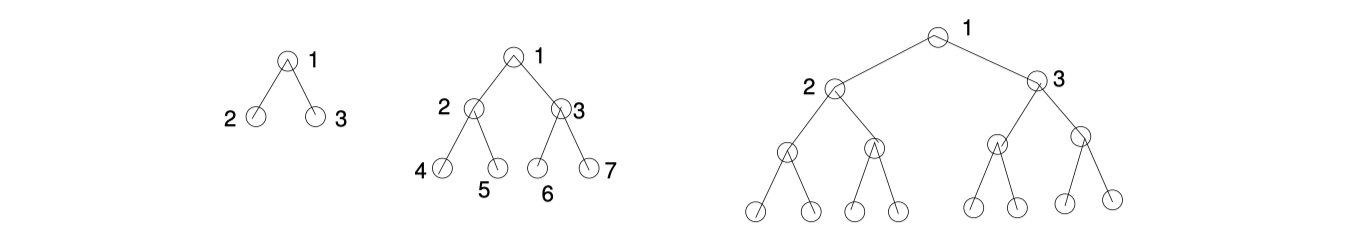
\includegraphics[width=1\linewidth]{Figs/tree.png}
\centering
\caption{$T_{1}, T_{2}$ and $T_{3}$. Node $1$ is at the top, $2$ and $3$ are its children. Some other nodes have been labeled as well.}
		\label{be:tree}
\end{figure}

\tb{upper bound of $\lambda_{2}$}

Let's first upper bound $\lambda_{2}\left(T_{d}\right)$ by constructing a test vector $x .$ Set $x(1)=0, x(2)=1$, and $x(3)=-1$. Then, for every vertex $u$ that we can reach from node 2 without going through node 1 , we set $x(u)=1$. For all the other nodes, we set $x(u)=-1$.

\begin{figure}[ht]
 \centering
 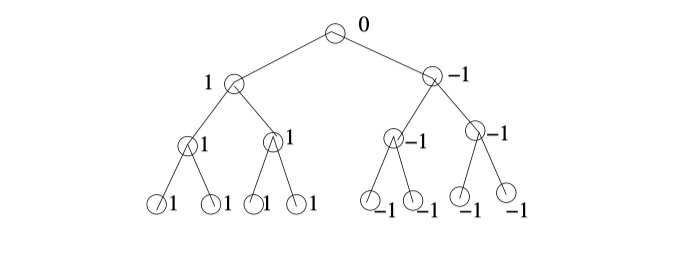
\includegraphics[width=0.5\linewidth]{Figs/tree_test.png}
\centering
\caption{The test vector we use to upper bound $\lambda_{2}\left(T_{3}\right)$.}
		\label{be:treetest}
\end{figure}

We then have
$$
\lambda_{2} \leq \frac{\sum_{(i, j) \in T_{d}}\left(x_{i}-x_{j}\right)^{2}}{\sum_{i} x_{i}^{2}}=\frac{\left(x_{1}-x_{2}\right)^{2}+\left(x_{1}-x_{3}\right)^{2}}{n-1}=2 /(n-1)
$$

\tb{lower bound of $\lambda_{2}$}

We will again prove a lower bound by comparing $T_{d}$ to the complete graph. For each edge $(i, j) \in$ $K_{n}$, let $T_{d}^{i, j}$ denote the unique path in $T$ from $i$ to $j$. This path will have length at most $2 d$. So, we have
$$
K_{n}=\sum_{i<j} G_{i, j} \preccurlyeq \sum_{i<j}(2 d) T_{d}^{i, j} \preccurlyeq \sum_{i<j}\left(2 \log _{2} n\right) T_{d}=\left(\begin{array}{c}
n \\
2
\end{array}\right)\left(2 \log _{2} n\right) T_{d}
$$
So, we obtain the bound
$$
\left(\begin{array}{l}
n \\
2
\end{array}\right)\left(2 \log _{2} n\right) \lambda_{2}\left(T_{d}\right) \geq n
$$
which implies
$$
\lambda_{2}\left(T_{d}\right) \geq \frac{1}{(n-1) \log _{2} n} .
$$

\section{Conductance, the Normalized Laplacian, and Cheeger’s Inequality}\label{sec:cnc}
\subsection{Definitions}
Let $G=(V,E)$, from \cref{lp:thmlower}, we know that for every $S \subset V$
$$
\theta(S) \geq \lambda_{2}(1-s)
$$
where $s=|S| /|V| .$. 


Re-arranging terms slightly, this can be stated as
$$
|V| \frac{|\partial(S)|}{|S||V-S|} \geq \lambda_{2}
$$
Cheeger's inequality provides a relation in the other direction. However, the relation is tighter and cleaner when we look at two slightly different quantities: the conductance of the set and the second eigenvalue of the normalized Laplacian.

\begin{defa}{\bfs{Conductance of Set of Vertex $S$}}
We definite conductance of $S$ to be
$$
\phi(S) \stackrel{\text { def }}{=} \frac{|\partial(S)|}{\min (d(S), d(V-S))},
$$
where $d(S)$ for the sum of the degrees of the vertices in $S$ ($d(S)$ is twice the number of edges in $S$).
\end{defa}
\begin{rema}
Note that many similar, although sometimes slightly different, definitions appear in the literature. For example, we would instead use
$$
\frac{d(V) \partial(S)}{d(S) d(V-S)}
$$ in \cref{lower:eqa}
\end{rema}
\begin{defa}{\bfs{Conductance of Graph $G$}}
We define the conductance of a graph $G$ to be
$$
\phi_{G} \stackrel{\text { def }}{=} \min _{S \subset V} \phi(S) \text { . }
$$
\end{defa}
\begin{rema}{\bfs{isoperimetric number vs. conductance}}
The conductance of a graph is more useful in many applications than the isoperimetric number. I usually find that conductance is the more useful quantity when you are concerned about edges, and that isoperimetric ratio is most useful when you are concerned about vertices. Conductance is particularly useful when studying random walks in graphs.
\end{rema}

\begin{defa}{\bfs{The Normalized Laplacian, $\boldsymbol{N}_G$}}For graph $G$, we define the normalized Laplacian of $G$ as 
$$
\boldsymbol{N}_G \coloneqq \boldsymbol{D}^{-1 / 2} \boldsymbol{L}_G \boldsymbol{D}^{-1 / 2}
$$
\end{defa} 
\begin{rema}{\bfs{how it comes}}Sometimes we care about the ratio:
$$
\frac{\boldsymbol{y}^{T} \boldsymbol{L} \boldsymbol{y}}{\boldsymbol{y}^{T} \boldsymbol{D} \boldsymbol{y}}
$$
If we make the change of variables
$$
\boldsymbol{D}^{1 / 2} \boldsymbol{y}=\boldsymbol{x}
$$
then this ratio becomes
$$
\frac{\boldsymbol{x}^{T} \boldsymbol{D}^{-1 / 2} \boldsymbol{L} \boldsymbol{D}^{-1 / 2} \boldsymbol{x}}{\boldsymbol{x}^{T} \boldsymbol{x}} .
$$
\end{rema}




We order the $n$ eigenvalue of the normalized Laplacian $\boldsymbol{N}_G$ as  $0=\nu_{1} \leq \nu_{2} \leq \cdots \leq \nu_{n}$.
The conductance is related to $\nu_{2}$ as the isoperimetric number is related to $\lambda_{2}$ which is shown in \cref{looo}.

\begin{rema}{\bfs{$\nu_{2}$ in terms of $
\frac{\boldsymbol{y}^{T} \boldsymbol{L} \boldsymbol{y}}{\boldsymbol{y}^{T} \boldsymbol{D} \boldsymbol{y}}
$}}\label{v2:aaa}

The eigenvector of eigenvalue $0$ of $\boldsymbol{N}$ is $\boldsymbol{d}^{1 / 2}$, where $\boldsymbol{d}^{1 / 2}(u)=\sqrt{d(u)}$, since we can observe that
$$
\boldsymbol{D}^{-1 / 2} \boldsymbol{L} \boldsymbol{D}^{-1 / 2} \boldsymbol{d}^{1 / 2}=\boldsymbol{D}^{-1 / 2} \boldsymbol{L} \mathbf{1}=\boldsymbol{D}^{-1 / 2} \mathbf{0}=\mathbf{0}
$$
The eigenvector of $\nu_{2}$ is given by
$$
\arg \min _{\bsl{x} \perp \bsl{d}^{1 / 2}} \frac{\boldsymbol{x}^{T} \boldsymbol{N} \boldsymbol{x}}{\boldsymbol{x}^{T} \boldsymbol{x}}
$$
Transfering back into the variable $\boldsymbol{y}$, and observing that
$$
\boldsymbol{x}^{T} \boldsymbol{d}^{1 / 2}=\boldsymbol{y}^{T} D^{1 / 2} \boldsymbol{d}^{1 / 2}=\boldsymbol{y}^{T} \boldsymbol{d}
$$
we find
$$
\nu_{2}=\min _{y \perp \bsl{d}} \frac{\boldsymbol{y}^{T} \boldsymbol{L} \boldsymbol{y}}{\boldsymbol{y}^{T} \boldsymbol{D} \boldsymbol{y}}
$$
\end{rema}


\begin{thma}{\bfs{Lower Bound on $\phi_{G}$ w.r.t. $\nu_{2}$}}\label{looo}
$$
\nu_{2} / 2 \leq \phi_{G}
$$
\end{thma}
\begin{proof}
As in the proof of \cref{lp:thmlower}, we would like to again use $\boldsymbol{\chi}_{S}$ as a test vector. But, it is not orthogonal to
d. To fix this, we subtrat a constant. Set
$$
\boldsymbol{y}=\boldsymbol{\chi}_{S}-\sigma \mathbf{1}
$$
where
$$
\sigma=d(S) / d(V)
$$
such that $\boldsymbol{y}^{T} \boldsymbol{d}=0$ :
$$
\boldsymbol{y}^{T} \boldsymbol{d}=\boldsymbol{\chi}_{S}^{T} \boldsymbol{d}-\sigma \mathbf{1}^{T} \boldsymbol{d}=d(S)-(d(S) / d(V)) d(V)=0
$$
We already know that
$$
\boldsymbol{y}^{T} \boldsymbol{L} \boldsymbol{y}=|\partial(S)|
$$
It remains to compute $\boldsymbol{y}^{T} \boldsymbol{D} \boldsymbol{y}$:
$$
\begin{aligned}
\boldsymbol{y}^{T} \boldsymbol{D} \boldsymbol{y} &=\sum_{u \in S} d(u)(1-\sigma)^{2}+\sum_{u \notin S} d(u) \sigma^{2} \\
&=d(S)(1-\sigma)^{2}+d(V-S) \sigma^{2} \\
&=d(S)-2 d(S) \sigma+d(V) \sigma^{2} \\
&=d(S)-d(S) \sigma \\
&=d(S) d(V-S) / d(V)
\end{aligned}
$$
So,
\begin{align}
    \nu_{2} \leq \frac{\boldsymbol{y}^{T} \boldsymbol{L} \boldsymbol{y}}{\boldsymbol{y}^{T} \boldsymbol{D} \boldsymbol{y}}=\frac{|\partial(S)| d(V)}{d(S) d(V-S)}
    \label{lower:eqa}
\end{align}
As the larger of $d(S)$ and $d(V-S)$ is at least half of $d(V)$, we find
$$
\nu_{2} \leq 2 \frac{|\partial(S)|}{\min (d(S), d(V-S))}
$$
\end{proof}

\subsection{Cheeger's inequality}

\begin{thma}{\bfs{Cheeger's inequality: Upper Bound on $\phi_{G}$ w.r.t. $\nu_{2}$}}\label{cheegerupper}
Let $y$ be a vector orthogonal to $\boldsymbol{d}$. Then, there is a number $t$ for which the set $S_{t}=\{u: \boldsymbol{y}(u)<t\}$ satisfies
\begin{align}
  \phi\left(S_{t}\right) \leq \sqrt{2 \frac{\boldsymbol{y}^{T} \boldsymbol{L} \boldsymbol{y}}{\boldsymbol{y}^{T} \boldsymbol{D} \boldsymbol{y}}} 
  \label{cheegerupper:eq1}
\end{align}


\end{thma} 
\begin{rema}{\bfs{rewrite as $\nu_{2}$}}From \cref{v2:aaa}, \cref{cheegerupper:eq1} actually tells us that 
$$
\phi_{G} \leq \sqrt{2 \nu_{2}}
$$
Cheeger's inequality proves that if we have a vector $\boldsymbol{y}$, orthogonoal to $\boldsymbol{d}$, then one can obtain a set of small conductance from $\boldsymbol{y}$. We obtain such a set by carefully choosing a real number $t$ in $S_t$
\end{rema}


Before proving \cref{cheegerupper},
we first show the denominator $\boldsymbol{y}^{T} \boldsymbol{D} \boldsymbol{y}$ in $\frac{\boldsymbol{y}^{T} \boldsymbol{L} \boldsymbol{y}}{\boldsymbol{y}^{T} \boldsymbol{D} \boldsymbol{y}}$ is essentially minimized when $\boldsymbol{y}^{T} \boldsymbol{d}=0$ with regards to shifts for a fixed $\boldsymbol{y}$.

\begin{lema}\label{mmmm}
Let $\boldsymbol{v}_{s}=\boldsymbol{y}+z \mathbf{1}$. Then, the minimum of $\boldsymbol{v}_{z}^{T} \boldsymbol{D} \boldsymbol{v}_{z}^{T}$ is achieved at the z for which $\boldsymbol{v}_{z}^{T} \boldsymbol{d}=0$
\end{lema}
\begin{proof}
The derivative with respect to $z$ is
$$
2 \boldsymbol{d}^{T} \boldsymbol{v}_{z}
$$
and the minimum is achieved when this derivative is zero.
\end{proof} 

\begin{proof}(of \cref{cheegerupper})
We begin our proof of Cheeger's inequality by defining
$$
\rho=\frac{\boldsymbol{y}^{T} \boldsymbol{L} \boldsymbol{y}}{\boldsymbol{y}^{T} \boldsymbol{D} \boldsymbol{y}}
$$
So, we need to show that there is a $t$ for which $\phi\left(S_{t}\right) \leq \sqrt{2 \rho}$.
By renumbering the vertices, we may assume without loss of generality that
$$
\boldsymbol{y}(1) \leq \boldsymbol{y}(2) \leq \cdots \leq \boldsymbol{y}(n)
$$
We begin with some normalization. Let $j$ be the least number for which
$$
\sum_{u=1}^{j} \boldsymbol{d}(u) \geq d(V) / 2
$$
We would prefer a vector that is centered at $j .$ So, set
$$
\boldsymbol{z}=\boldsymbol{y}-\boldsymbol{y}(j) \mathbf{1}
$$
This vector $\boldsymbol{z}$ satisfies $\boldsymbol{z}(j)=0$. Since $\boldsymbol{d}^T\boldsymbol{y}=0$, by \cref{mmmm},
$$
\frac{\boldsymbol{z}^{T} \boldsymbol{L} \boldsymbol{z}}{\boldsymbol{z}^{T} \boldsymbol{D} \boldsymbol{z}} \leq \rho
$$
We also multiply $\boldsymbol{z}$ by a constant ($\frac{\boldsymbol{z}^{T} \boldsymbol{L} \boldsymbol{z}}{\boldsymbol{z}^{T} \boldsymbol{D} \boldsymbol{z}}$ is not changed) so that
$$
z(1)^{2}+z(n)^{2}=1
$$
Recall that
$$
\phi(S)=\frac{|\partial(S)|}{\min (d(S), d(V-S))}
$$
\tb{Key:}

We will define a distribution on $t$ for which we can prove that
$$
\mathbb{E}\left[\left|\partial\left(S_{t}\right)\right|\right] \leq \sqrt{2 \rho} \mathbb{E}\left[\min \left(d\left(S_{t}\right), d\left(V-S_{t}\right)\right)\right]
$$
This implies that there is some $t$ for which
$$
\left|\partial\left(S_{t}\right)\right| \leq \sqrt{2 \rho} \min \left(d\left(S_{t}\right), d\left(V-S_{t}\right)\right)
$$
which means $\phi(S) \leq \sqrt{2 \rho}$.


To switch from working with $\boldsymbol{y}$ to working with $\boldsymbol{z}$, define We will set $$S_{t}=\{u: \boldsymbol{z}(u) \leq t\}.$$ 
\tb{Solution: the constructed distribution}

Trevisan had the remarkable idea of choosing $t$ between $\boldsymbol{z}(1)$ and $\boldsymbol{z}(n)$ with probability density $2|t| .$ That is, the probability that $t$ lies in the interval $[a, b]$ is
$$
\int_{t=a}^{b} 2|t| .
$$
To see that the total probability is $1$, observe that
$$
\int_{t=\bsl{z}(1)}^{z(n)} 2|t|=\int_{t=\bsl{z}(1)}^{0} 2|t|+\int_{t=0}^{\bsl{z}(n)} 2|t|=\boldsymbol{z}(n)^{2}+\boldsymbol{z}(1)^{2}=1
$$
as $\boldsymbol{z}(1) \leq \boldsymbol{z}(j) \leq \boldsymbol{z}(n)$ and $\boldsymbol{z}(j)=0$
Similarly, the probability that $t$ lies in the interval $[a, b]$ is
$$
\int_{t=a}^{b} 2|t|=\operatorname{sgn}(b) b^{2}-\operatorname{sgn}(a) a^{2},
$$
where
$$
\operatorname{sgn}(x)=\left\{\begin{array}{ll}
1 & \text { if } x>0 \\
0 & \text { if } x=0, \text { and } \\
-1 & \text { if } x<0
\end{array}\right.
$$
\tb{1. A bound for $\mathbb{E}_{t}\left[\left|\partial\left(S_{t}\right)\right|\right]$:}
\begin{align}
 \mathbb{E}_{t}\left[\left|\partial\left(S_{t}\right)\right|\right]=\sum_{(u, v) \in E} \P_{t}\left[(u, v) \in \partial\left(S_{t}\right)\right] \leq \sum_{(u, v) \in E}|z(u)-\boldsymbol{z}(v)|(|\boldsymbol{z}(u)|+|\boldsymbol{z}(v)|)   \label{eq:dd1}
\end{align}
Proof of the bound: An edge $(u, v)$ with $\boldsymbol{z}(u) \leq \boldsymbol{z}(v)$ is on the boundary of $S$ if
$$
\boldsymbol{z}(u) \leq t<\boldsymbol{z}(v)
$$
The probability that this happens is
$$
\operatorname{sgn}(\boldsymbol{z}(v)) \boldsymbol{z}(v)^{2}-\operatorname{sgn}(\boldsymbol{z}(u)) \boldsymbol{z}(u)^{2}=\left\{\begin{array}{ll}
\left|\boldsymbol{z}(u)^{2}-\boldsymbol{z}(v)^{2}\right| & \text { when } \operatorname{sgn}(\bsl{z}(u))=\operatorname{sgn}(\bsl{z}(v)) \\
\boldsymbol{z}(u)^{2}+\boldsymbol{z}(v)^{2} & \text { when } \operatorname{sgn}(\bsl{z}(u)) \neq \operatorname{sgn}(\bsl{z}(v))
\end{array}\right.
$$
We now show that both of these terms are upper bounded by
$$
|\boldsymbol{z}(u)-\boldsymbol{z}(v)|(|\boldsymbol{z}(u)|+|\boldsymbol{z}(v)|)
$$
Regardless of the signs,
$$
\left|\boldsymbol{z}(u)^{2}-\boldsymbol{z}(v)^{2}\right|=|(\boldsymbol{z}(u)-\boldsymbol{z}(v))(\boldsymbol{z}(u)+\boldsymbol{z}(v))| \leq|\boldsymbol{z}(u)-\boldsymbol{z}(v)|(|\boldsymbol{z}(u)|+|\boldsymbol{z}(v)|)
$$
When $\operatorname{sgn}(\bsl{u})=-\operatorname{sgn}(\bsl{v})$
$$
\boldsymbol{z}(u)^{2}+\boldsymbol{z}(v)^{2} \leq(\boldsymbol{z}(u)-\boldsymbol{z}(v))^{2}=|\boldsymbol{z}(u)-\boldsymbol{z}(v)|(|\boldsymbol{z}(u)|+|\boldsymbol{z}(v)|) .
$$

\tb{2. A new formulation of expected denominator of $\phi$:}
$$
\E{t}\left[\min \left(d\left(S_{t}\right), d\left(V-S_{t}\right)\right)\right]=\boldsymbol{z}^{T} \boldsymbol{D} \boldsymbol{z}
$$
Proof of the new formulation: Observe that
$$
\mathbb{E}_{t}\left[d\left(S_{t}\right)\right]=\sum_{u} \P_{t}\left[u \in S_{t}\right] d(u)=\sum_{u} \P_{t}[\boldsymbol{z}(u) \leq t] d(u)
$$
The result of our centering of $z$ at $j$ is that
$$
\begin{array}{l}
t<0 \Longrightarrow d(S_t)=\min (d(S_t), d(V-S_t)), \quad \text { and } \\
t \geq 0 \Longrightarrow d(V-S_t)=\min (d(S_t), d(V-S_t))
\end{array}
$$
That is, for $u<j, u$ is in the smaller set if $t<0$; and, for $u \geq j, u$ is in the smaller set if $t \geq 0$. So,
$$
\begin{aligned}
\mathbb{E}_{t}\left[\min \left(d\left(S_{t}\right), d\left(V-S_{t}\right)\right)\right] &=\sum_{u<j} \P[\boldsymbol{z}(u)<t \text { and } t<0] d(u)+\sum_{u \geq j} \P[\boldsymbol{z}(u)>t \text { and } t \geq 0] d(u) \\
&=\sum_{u<j} \P[\boldsymbol{z}(u)<t<0] d(u)+\sum_{u \geq j} \P[\boldsymbol{z}(u)>t \geq 0] d(u) \\
&=\sum_{u<j} \boldsymbol{z}(u)^{2} d(u)+\sum_{u \geq j} \boldsymbol{z}(u)^{2} d(u) \\
&=\sum_{u} \boldsymbol{z}(u)^{2} d(u) \\
&=\boldsymbol{z}^{T} \boldsymbol{D} \boldsymbol{z}
\end{aligned}
$$

\tb{3. Final step: an application of Cauchy-Schwartz inequality:}

Recall that our goal is to prove that
$$
\mathbb{E}\left[\left|\partial\left(S_{t}\right)\right|\right] \leq \sqrt{2 \rho} \mathbb{E}\left[\min \left(d\left(S_{t}\right), d\left(V-S_{t}\right)\right)\right]
$$
and we know that
$$
\E{t}\left[\min \left(d\left(S_{t}\right), d\left(V-S_{t}\right)\right)\right]=\sum_{u} \boldsymbol{z}(u)^{2} d(u)
$$
and that
$$
\mathbb{E}_{t}\left[\left|\partial\left(S_{t}\right)\right|\right] \leq \sum_{(u, v) \in E}|\boldsymbol{z}(u)-\boldsymbol{z}(v)|(|\boldsymbol{z}(u)|+|\boldsymbol{z}(v)|)
$$
We may use the Cauchy-Schwartz inequality to upper bound the term above by
\begin{align}
    \sqrt{\sum_{(u, v) \in E}(\boldsymbol{z}(u)-\boldsymbol{z}(v))^{2}} \sqrt{\sum_{(u, v) \in E}(|\boldsymbol{z}(u)|+|\boldsymbol{z}(v)|)^{2}}\label{eq:dd}
\end{align}



We have defined $\rho$ so that the term under the left-hand square root is at most
$$
\rho \sum_{u} \boldsymbol{z}(u)^{2} d(u)
$$
To bound the right-hand square root, we observe
$$
\sum_{(u, v) \in E}(|\boldsymbol{z}(u)|+|\boldsymbol{z}(v)|)^{2} \leq 2 \sum_{(u, v) \in E} \boldsymbol{z}(u)^{2}+\boldsymbol{z}(v)^{2}=2 \sum_{u} \boldsymbol{z}(u)^{2} d(u)
$$
Putting all these inequalities together yields
$$
\begin{aligned}
\mathbb{E}[|\partial(S)|] & \leq \sqrt{\rho \sum_{u} \boldsymbol{z}(u)^{2} d(u)} \sqrt{2 \sum_{u} \boldsymbol{z}(u)^{2} d(u)} \\
&=\sqrt{2 \rho} \sum_{u} \boldsymbol{z}(u)^{2} d(u) \\
&=\sqrt{2 \rho} \mathbb{E}[\min (d(S), d(V-S))]
\end{aligned}
$$
\end{proof}
\begin{rema}
I wish to point out two important features of this proof
\begin{enumerate}
    \item This proof does not require $\bsl{y}$ to be an eigenvector, we just require any $\bsl{y}$ that is orthogonal to $\boldsymbol{d}$.
    \item This proof goes through almost without change for weighted graphs. The main difference is that for weighted graphs we measure the sum of the weights of edges on the boundary instead of their number. The main difference in the proof is that lines \cref{eq:dd1} and \cref{eq:dd} become
$$
\begin{aligned}
\mathbb{E}[w(\partial(S))] &=\sum_{(u, v) \in E} \P[(u, v) \in \partial(S)] w_{u, v} \\
& \leq \sum_{(u, v) \in E}|\boldsymbol{z}(u)-\boldsymbol{z}(v)|(|\boldsymbol{z}(u)|+|\boldsymbol{z}(v)|) w_{u, v} \\
& \leq \sqrt{\sum_{(u, v) \in E} w_{u, v}(\boldsymbol{z}(u)-\boldsymbol{z}(v))^{2}} \sqrt{\sum_{(u, v) \in E} w_{u, v}(|\boldsymbol{z}(u)|+|\boldsymbol{z}(v)|)^{2}}
\end{aligned}
$$
and we observe that
$$
\sum_{(u, v) \in E} w_{u, v}(|\boldsymbol{z}(u)|+|\boldsymbol{z}(v)|)^{2} \leq 2 \sum_{u} \boldsymbol{z}(u)^{2} d(u)
$$
\end{enumerate}
\end{rema}




\bibliographystyle{IEEEtran}
\bibliography{IEEEabrv,StringDefinitions,adv_dnn}
\end{document}
